\section{יחידה 9: ההתפלגות הנורמלית}

יחידה זו עוסקת בהתפלגות הנורמלית, שהיא מודל תאורטי מרכזי בסטטיסטיקה.
הדגש הוא על הבנת צורת ההתפלגות, משמעות הפרמטרים שלה, והקשר בין שטח תחת העקומה להסתברות.



\subsection{מהי התפלגות נורמלית}

התפלגות נורמלית היא התפלגות רציפה, סימטרית ופעמונית, המתוארת על ידי שני פרמטרים:
\begin{itemize}
\item $\mu$ – תוחלת (ממוצע)
\item $\sigma$ – סטיית תקן
\end{itemize}

\subsubsection{מאפיינים מרכזיים}
\begin{itemize}
\item סימטריה סביב $\mu$
\item ממוצע = חציון = שכיח
\item זנבות אינסופיים (אך השכיחות בהם קטנה מאוד)
\end{itemize}



\subsection{משמעות הפרמטרים}

\subsubsection{התוחלת $\mu$}
קובעת את מיקום ההתפלגות על ציר ה־$X$.

\subsubsection{סטיית התקן $\sigma$}
קובעת את פיזור ההתפלגות:
\begin{itemize}
\item $\sigma$ גדולה → התפלגות רחבה ושטוחה
\item $\sigma$ קטנה → התפלגות צרה וגבוהה
\end{itemize}



\subsection{שטח כהסתברות}

\subsubsection{פונקציית צפיפות אינה הסתברות}

פונקציית הצפיפות $f(x)$ אינה נותנת הסתברות לערך בודד.
היא מתארת את \textbf{קצב הצטברות ההסתברות} סביב ערך מסוים.

באופן פורמלי:
\begin{english}
\[
f(x)
=
\lim_{\Delta x \to 0}
\frac{P(x \le X < x+\Delta x)}{\Delta x}
\]
\end{english}

לכן:
\begin{itemize}
\item $f(x)$ יכולה להיות גדולה מ־1
\item $f(x)$ אינה הסתברות
\item רק \textbf{שטח} מתחת לגרף מייצג הסתברות
\end{itemize}

בהתפלגות נורמלית:
\[
\text{השטח מתחת לעקומה} = \text{הסתברות}
\]

\subsubsection{דגשים}
\begin{itemize}
\item סך כל השטח = 1
\item הסתברות לערך בודד = 0
נקודה היא קטע באורך אפס, ולכן השטח שלה אפס.
אין מדובר באירוע בלתי אפשרי, אלא באירוע חסר משקל הסתברותי.
\item מחשבים הסתברויות רק עבור תחומים
\end{itemize}

\subsubsection{הסבר מתמטי: הסתברות לערך בודד}

במשתנה מקרי רציף:
\begin{english}
\[
P(X = x_0) = \int_{x_0}^{x_0} f(x)\,dx = 0
\]
\end{english}

\subsubsection{מדידה בפועל מול המודל הרציף}

למרות שבמודל הרציף ההסתברות לערך בודד היא אפס,
בפועל כל מדידה מניבה ערך מספרי יחיד.

הסיבה לכך היא שכל מדידה מתבצעת בדיוק סופי,
ולכן ערך מדוד מייצג בפועל טווח קטן של ערכים:
\begin{english}
\[
x_0 - \varepsilon \le X < x_0 + \varepsilon
\]
\end{english}

לטווח כזה יש אורך חיובי ולכן הסתברות חיובית.

\subsubsection{שוויון בין $<$ ל־$\le$ במשתנה רציף}

במשתנה מקרי רציף מתקיים:
\begin{english}
\[
P(X \le a) = P(X < a)
\]
\end{english}

הסיבה:
\begin{english}
\[
P(X \le a) = P(X < a) + P(X = a)
\]
\end{english}

ומכיוון ש־$P(X=a)=0$, אין הבדל בין הסימנים.

\subsection{כלל האצבע (68–95–99.7)}

\begin{itemize}
\item כ־68\% מהתצפיות בתחום $\mu \pm \sigma$
\item כ־95\% בתחום $\mu \pm 2\sigma$
\item כ־99.7\% בתחום $\mu \pm 3\sigma$
\end{itemize}

\subsubsection{דגש למבחן}
כלל האצבע הוא \textbf{קירוב}, לא חישוב מדויק.



\subsection{תקנון}

\subsubsection{הרעיון}
המרה של משתנה נורמלי כללי למשתנה נורמלי סטנדרטי.

\[
Z = \frac{X - \mu}{\sigma}
\]

\subsubsection{שימור הסתברויות תחת תקנון}

התקנון הוא טרנספורמציה לינארית שאינה משנה הסתברויות אלא רק את סולם המדידה.

לכן מתקיים:
\begin{english}
\[
P(a \le X \le b)
=
P\left(
\frac{a-\mu}{\sigma}
\le Z \le
\frac{b-\mu}{\sigma}
\right)
\]
\end{english}

המשמעות:
\begin{itemize}
\item האזורים משתנים בציר $X$
\item אך השטח (ההסתברות) נשמר
\end{itemize}
\textbf{דגש:} התקנון אינו משנה את סדר הערכים ולכן אינו משנה אחוזונים.


\subsection{ההתפלגות הנורמלית הסטנדרטית}

מסומנת $Z \sim N(0,1)$.

\subsubsection{למה מתקננים}
\begin{itemize}
\item כדי להשתמש בטבלת Z
\item כדי להשוות בין משתנים שונים
\end{itemize}

\subsection{טבלת Z (ראו נספח)}
טבלת Z מופיעה בנספח ומשמשת לחישוב שטחים בהתפלגות הנורמלית הסטנדרטית.

טבלת Z נותנת את השטח מהממוצע ($0$) ועד לערך $Z$ בעמודה B.
כדי לקבל את השטח הכולל משמאל ל־$Z$ חיובי מחשבים:
\[
P(Z < z) = 0.5 + B
\]

\subsubsection{קריאה בסיסית}
\begin{itemize}
\item שורה – ספרות שלמות + עשירית
\item עמודה – מאיות
\end{itemize}



\subsection{מקרים קלאסיים לחישוב}

\subsubsection{מתחת לערך}
\[
P(Z < z) \Rightarrow \text{ישירות מהטבלה}
\]

\subsubsection{מעל לערך}
\[
P(Z > z) = 1 - P(Z < z)
\]

\subsubsection{בין שני ערכים}
\[
P(z_1 < Z < z_2) = P(Z < z_2) - P(Z < z_1)
\]

\subsubsection{סימטריה}
\[
P(Z < -z) = 1 - P(Z < z)
\]



\subsection{אחוזונים בהתפלגות נורמלית}

\subsubsection{רעיון}
אחוזון הוא ערך שמתחתיו נמצאים $p\%$ מהנתונים.

\subsubsection{שימוש בטבלה}
\begin{itemize}
\item מוצאים בטבלה שטח קרוב ל־$p$
\item קוראים את ערך $Z$
\item מבצעים תקנון הפוך:
\[
X = \mu + Z\sigma
\]
\end{itemize}

\subsection{המחשה גרפית של ההתפלגות הנורמלית}
התפלגות נורמלית היא סימטרית ובעלת צורת פעמון. השטח מתחת לעקומה מייצג הסתברות.

[Image of normal distribution curve with standard deviations and percentages]

\begin{figure}[H]
\centering
\begin{english} % זה מה שימרכז את הגרף חזרה לדף
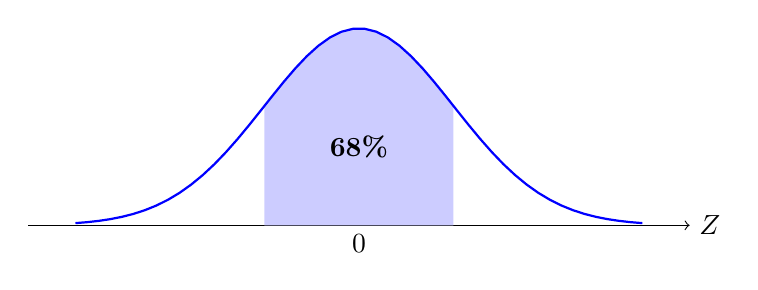
\begin{tikzpicture}[xscale=1.2, yscale=2.5]
  \draw[->] (-3.5,0) -- (3.5,0) node[right] {$Z$};
  \fill[blue!20] (-1,0) -- plot[domain=-1:1, samples=20] (\x, {exp(-(\x*\x)/2)}) -- (1,0) -- cycle;
  \draw[thick, blue, domain=-3:3, samples=50] plot (\x, {exp(-(\x*\x)/2)});
  \node at (0,0.4) {\textbf{68\%}};
  \node[below] at (0,0) {0};
\end{tikzpicture}
\end{english}
\caption{התפלגות נורמלית וכלל האצבע.}
\end{figure}

\subsection{טעויות נפוצות במבחן}

\begin{itemize}
\item לשכוח ש־Z-table נותנת שטח משמאל
\item להתבלבל בין מעל ומתחת
\item לא לבצע תקנון לפני שימוש בטבלה
\item לחשוב שכל משתנה הוא נורמלי
\end{itemize}



\subsection{דגש מסכם ליחידה}

לפני חישוב:
\begin{enumerate}
\item האם המשתנה נורמלי?
\item האם צריך תקנון?
\item איזה שטח מחפשים?
\item האם צריך להשתמש בסימטריה?
\end{enumerate}
